%%%%%%%%%%%%%%%%%%%%%%%%%%%%%%%%%%%%%%%%%%%%%%%%%%%
\begin{frame}
  \begin{center}
    {\Large CNN using PyTorch}
    
  \end{center}
  
  \tiny{(Ref: PyTorch Zero To All Lecture by Sung Kim)}
\end{frame}


%%%%%%%%%%%%%%%%%%%%%%%%%%%%%%%%%%%%%%%%%%%%%%%%%%%
\begin{frame}[fragile] \frametitle{CNN}
\begin{center}
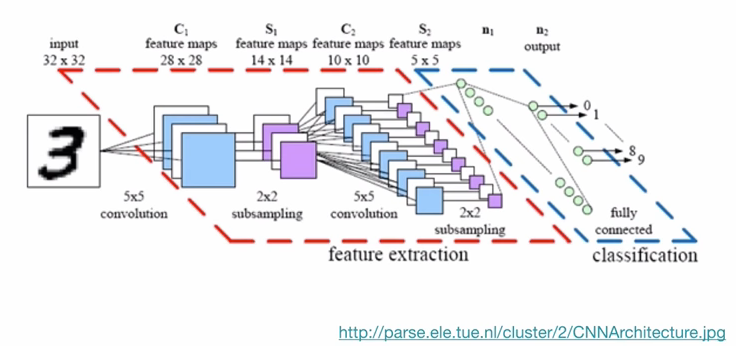
\includegraphics[width=0.8\linewidth,keepaspectratio]{pyhun42}
\end{center}
First few layers are convoution+subsampling and at the end dense
\end{frame}


%%%%%%%%%%%%%%%%%%%%%%%%%%%%%%%%%%%%%%%%%%%%%%%%%%%
\begin{frame}[fragile] \frametitle{Convolution}
\begin{center}
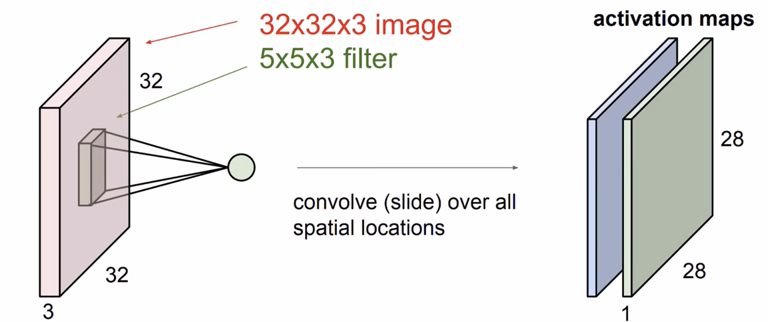
\includegraphics[width=0.8\linewidth,keepaspectratio]{pyhun43}
\end{center}
Looking at small portion of image, generating feature maps, one for each filter.
\end{frame}

%%%%%%%%%%%%%%%%%%%%%%%%%%%%%%%%%%%%%%%%%%%%%%%%%%%
\begin{frame}[fragile] \frametitle{Convolution}
\begin{center}
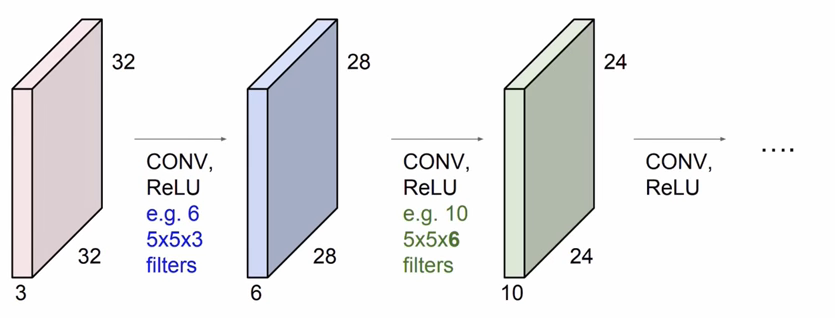
\includegraphics[width=0.8\linewidth,keepaspectratio]{pyhun44}
\end{center}
First layer had 6 filters and the second has 10.
\end{frame}


%%%%%%%%%%%%%%%%%%%%%%%%%%%%%%%%%%%%%%%%%%%%%%%%%%%
\begin{frame}[fragile] \frametitle{Pooling/Sub-sampling}
\begin{center}
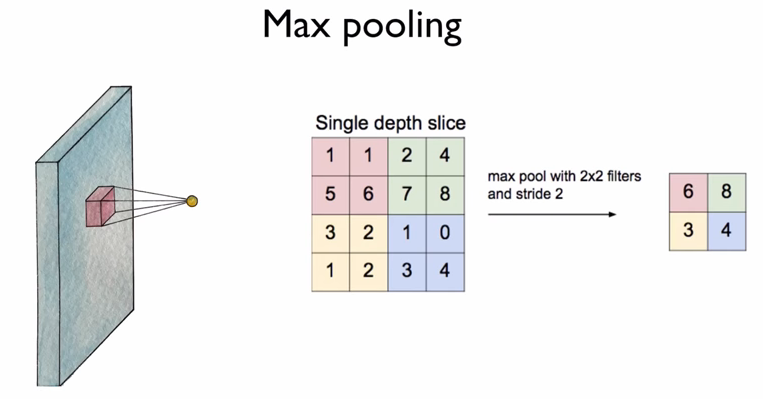
\includegraphics[width=0.8\linewidth,keepaspectratio]{pyhun45}
\end{center}

\end{frame}


%%%%%%%%%%%%%%%%%%%%%%%%%%%%%%%%%%%%%%%%%%%%%%%%%%%
\begin{frame}[fragile] \frametitle{Difference}
\begin{center}
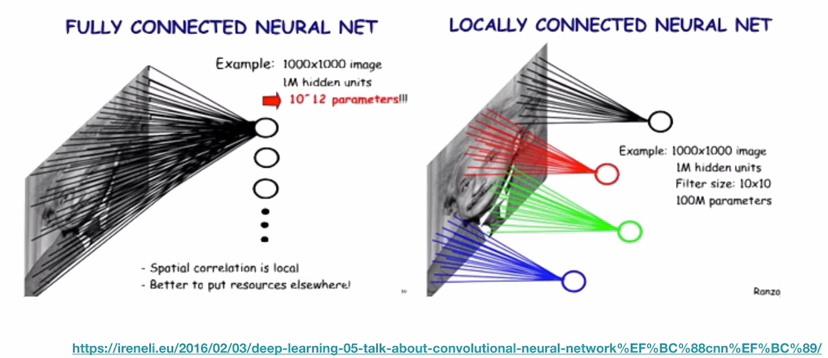
\includegraphics[width=0.8\linewidth,keepaspectratio]{pyhun46}
\end{center}
CNN is more flexible as it looks are smaller data, so smaller weights.
\end{frame}


%%%%%%%%%%%%%%%%%%%%%%%%%%%%%%%%%%%%%%%%%%%%%%%%%%%
\begin{frame}[fragile] \frametitle{Simple CNN for MNIST}
\begin{center}
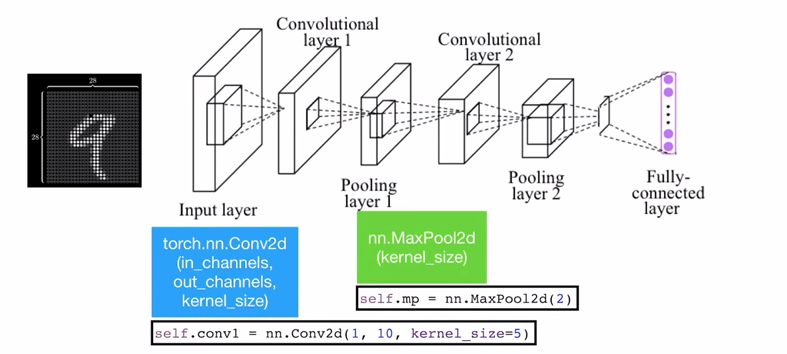
\includegraphics[width=0.8\linewidth,keepaspectratio]{pyhun47}
\end{center}
Using ready Conv2d layer with 1 input channel (greyscale), output channel = 10 (labels).
\end{frame}


%%%%%%%%%%%%%%%%%%%%%%%%%%%%%%%%%%%%%%%%%%%%%%%%%%%
\begin{frame}[fragile] \frametitle{Simple CNN for MNIST}
\begin{center}
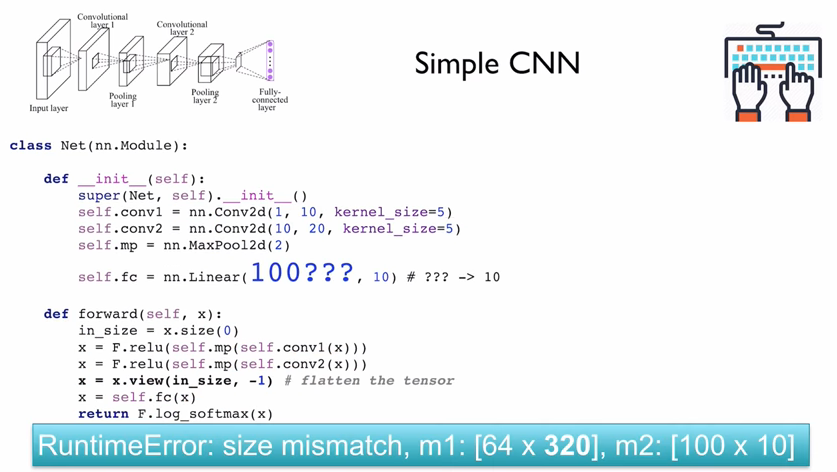
\includegraphics[width=0.8\linewidth,keepaspectratio]{pyhun48}
\end{center}

Outputs and Inputs need to be adjusted properly.  Calculating size after second pooling is not trivial, so just put some value and run. You will get error, suggesting a correct value. 64 is batch size, 320 is the flattened vector. Put 320 there.
\end{frame}

%%%%%%%%%%%%%%%%%%%%%%%%%%%%%%%%%%%%%%%%%%%%%%%%%%%
\begin{frame}[fragile] \frametitle{Simple CNN for MNIST}
\begin{center}
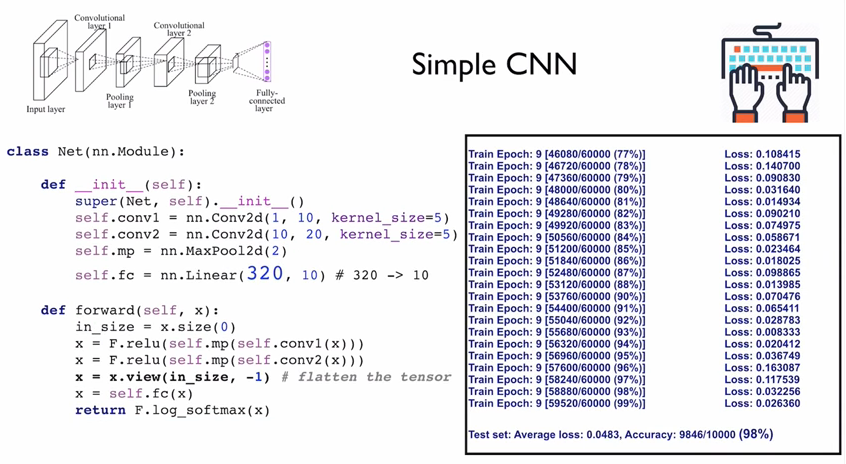
\includegraphics[width=\linewidth,keepaspectratio]{pyhun49}
\end{center}


\end{frame}






%%%%%%%%%%%%%%%%%%%%%%%%%%%%%%%%%%%%%%%%%%%%%%%%%%%
\begin{frame}
  \begin{center}
    {\Large CNN using PyTorch: Comprehensive}
    
\tiny{(Ref: Pytorch Official documentation + few other sources, like Lyman Lin (NTU)))}
  \end{center}
\end{frame}



%%%%%%%%%%%%%%%%%%%%%%%%%%%%%%%%%%%%%%%%%%%%%%%%%%%
\begin{frame}[fragile] \frametitle{How CNN Works}
\begin{center}
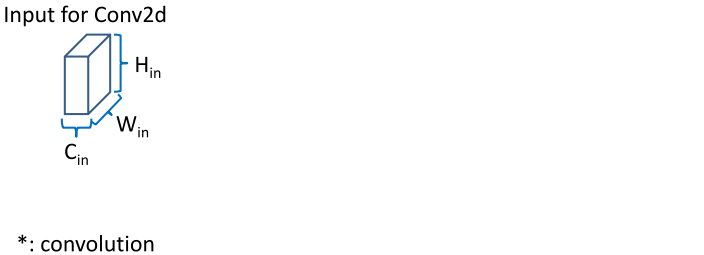
\includegraphics[width=0.8\linewidth,keepaspectratio]{pyt20}
\end{center}

\end{frame}

%%%%%%%%%%%%%%%%%%%%%%%%%%%%%%%%%%%%%%%%%%%%%%%%%%%
\begin{frame}[fragile] \frametitle{How CNN Works}
\begin{center}
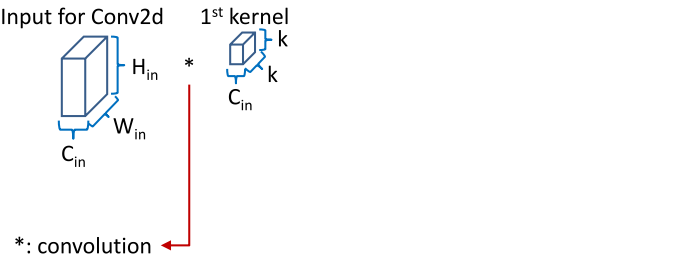
\includegraphics[width=0.8\linewidth,keepaspectratio]{pyt21}
\end{center}

\end{frame}

%%%%%%%%%%%%%%%%%%%%%%%%%%%%%%%%%%%%%%%%%%%%%%%%%%%
\begin{frame}[fragile] \frametitle{How CNN Works}
\begin{center}
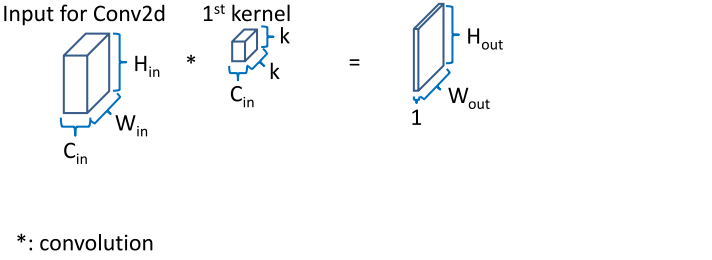
\includegraphics[width=0.8\linewidth,keepaspectratio]{pyt22}
\end{center}

\end{frame}

%%%%%%%%%%%%%%%%%%%%%%%%%%%%%%%%%%%%%%%%%%%%%%%%%%%
\begin{frame}[fragile] \frametitle{How CNN Works}
\begin{center}
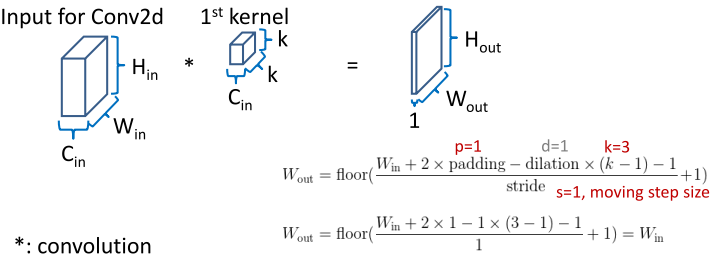
\includegraphics[width=0.8\linewidth,keepaspectratio]{pyt23}
\end{center}

\end{frame}

%%%%%%%%%%%%%%%%%%%%%%%%%%%%%%%%%%%%%%%%%%%%%%%%%%%
\begin{frame}[fragile] \frametitle{How CNN Works}
\begin{center}
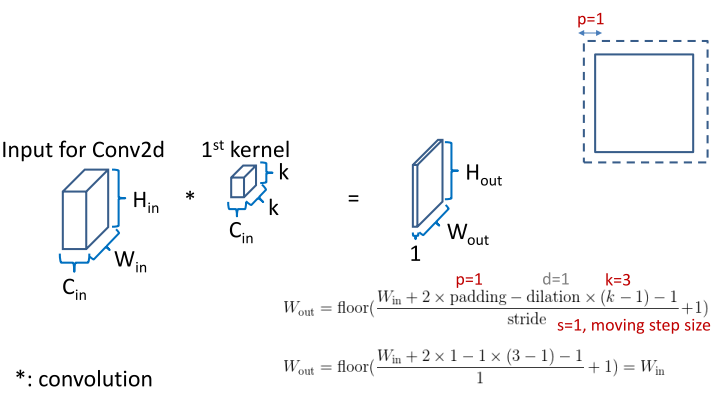
\includegraphics[width=0.8\linewidth,keepaspectratio]{pyt24}
\end{center}

\end{frame}

%%%%%%%%%%%%%%%%%%%%%%%%%%%%%%%%%%%%%%%%%%%%%%%%%%%
\begin{frame}[fragile] \frametitle{How CNN Works}
\begin{center}
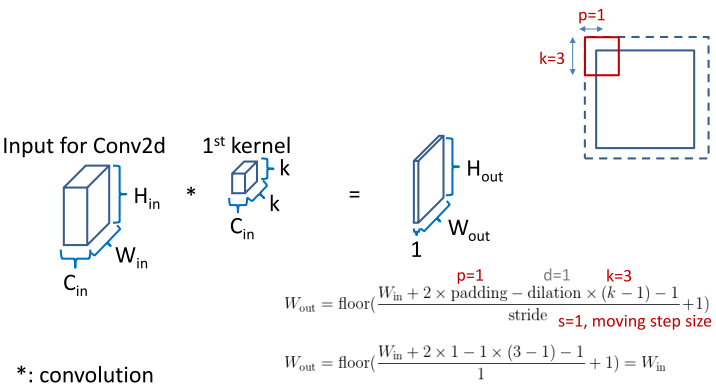
\includegraphics[width=0.8\linewidth,keepaspectratio]{pyt25}
\end{center}

\end{frame}

%%%%%%%%%%%%%%%%%%%%%%%%%%%%%%%%%%%%%%%%%%%%%%%%%%%
\begin{frame}[fragile] \frametitle{How CNN Works}
\begin{center}
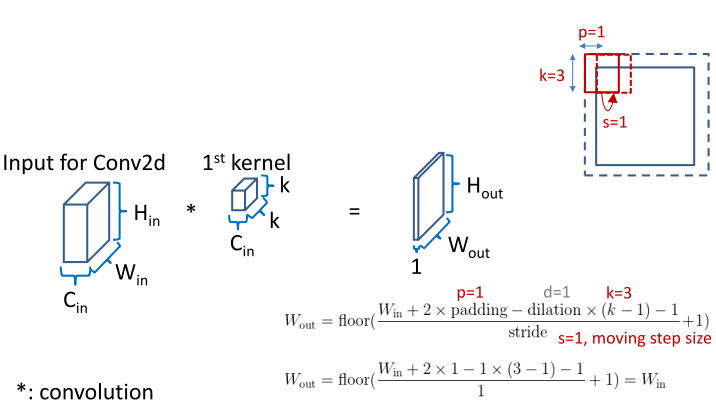
\includegraphics[width=0.8\linewidth,keepaspectratio]{pyt26}
\end{center}

\end{frame}

%%%%%%%%%%%%%%%%%%%%%%%%%%%%%%%%%%%%%%%%%%%%%%%%%%%
\begin{frame}[fragile] \frametitle{How CNN Works}
\begin{center}
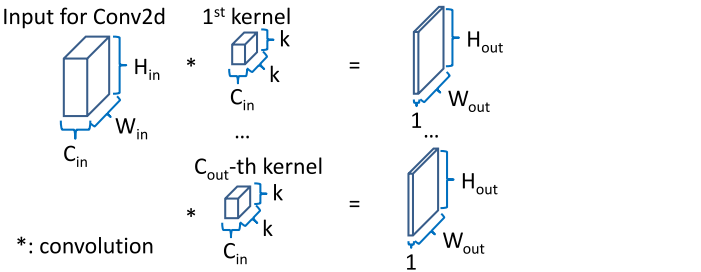
\includegraphics[width=0.8\linewidth,keepaspectratio]{pyt27}
\end{center}

\end{frame}


%%%%%%%%%%%%%%%%%%%%%%%%%%%%%%%%%%%%%%%%%%%%%%%%%%%
\begin{frame}[fragile] \frametitle{How CNN Works}
\begin{center}
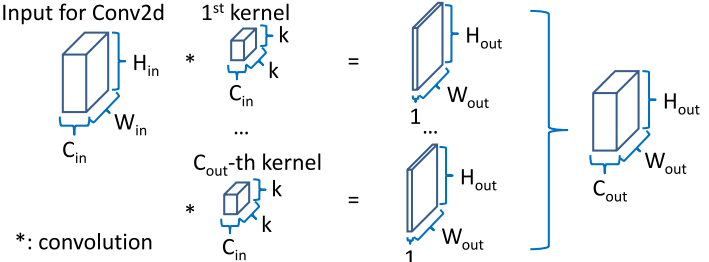
\includegraphics[width=0.8\linewidth,keepaspectratio]{pyt28}
\end{center}

\end{frame}
%%%%%%%%%%%%%%%%%%%%%%%%%%%%%%%%%%%%%%%%%%%%%%%%%%%
\begin{frame}[fragile] \frametitle{How CNN Works}
\begin{center}
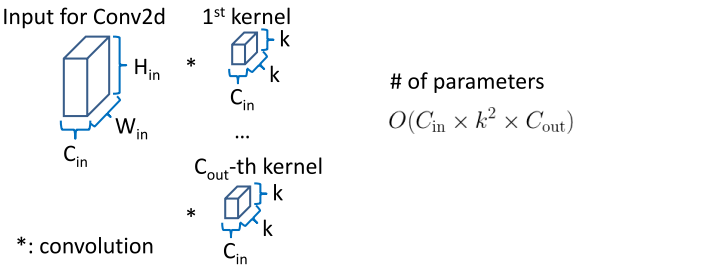
\includegraphics[width=0.8\linewidth,keepaspectratio]{pyt29}
\end{center}

\end{frame}


%%%%%%%%%%%%%%%%%%%%%%%%%%%%%%%%%%%%%%%%%%%%%%%%%%%
\begin{frame}[fragile] \frametitle{How CNN Works}
\begin{center}
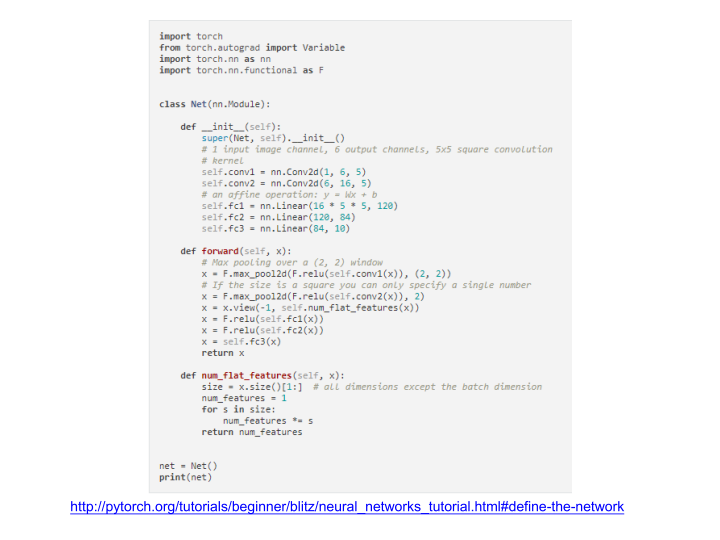
\includegraphics[width=0.8\linewidth,keepaspectratio]{pyt6}
\end{center}

\end{frame}

%%%%%%%%%%%%%%%%%%%%%%%%%%%%%%%%%%%%%%%%%%%%%%%%%%%
\begin{frame}[fragile] \frametitle{How CNN Works}
\begin{center}
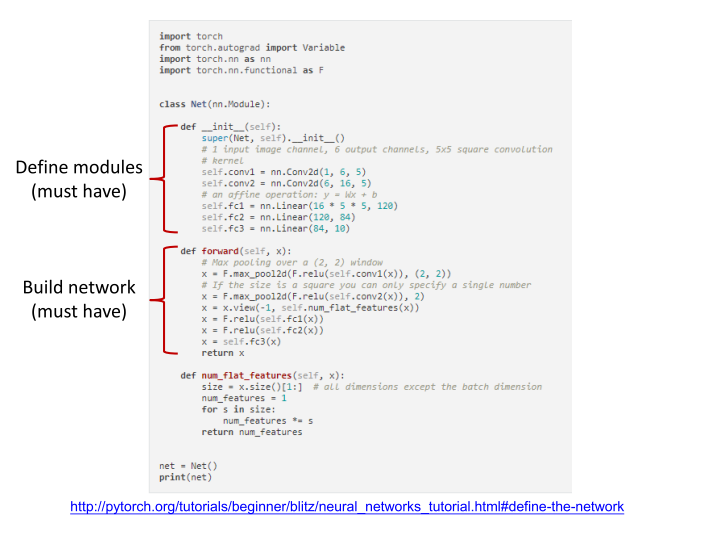
\includegraphics[width=0.8\linewidth,keepaspectratio]{pyt7}
\end{center}

\end{frame}


%%%%%%%%%%%%%%%%%%%%%%%%%%%%%%%%%%%%%%%%%%%%%%%%%%%
\begin{frame}[fragile] \frametitle{Define the network}
\begin{lstlisting}
import torch
from torch.autograd import Variable
import torch.nn as nn
import torch.nn.functional as F

class Net(nn.Module):
	pass
	
net = Net()
print(net)
\end{lstlisting}
\end{frame}

%%%%%%%%%%%%%%%%%%%%%%%%%%%%%%%%%%%%%%%%%%%%%%%%%%%
\begin{frame}[fragile] \frametitle{Define the network}
\begin{lstlisting}
class Net(nn.Module):

    def __init__(self):
        super(Net, self).__init__()
        # 1 input image channel, 6 output channels, 5x5 square convolution
        # kernel
        self.conv1 = nn.Conv2d(1, 6, 5)
        self.conv2 = nn.Conv2d(6, 16, 5)
        # an affine operation: y = Wx + b
        self.fc1 = nn.Linear(16 * 5 * 5, 120)
        self.fc2 = nn.Linear(120, 84)
        self.fc3 = nn.Linear(84, 10)
\end{lstlisting}
\end{frame}



%%%%%%%%%%%%%%%%%%%%%%%%%%%%%%%%%%%%%%%%%%%%%%%%%%%
\begin{frame}[fragile] \frametitle{Define the network}
\begin{lstlisting}
class Net(nn.Module):

    def forward(self, x):
        # Max pooling over a (2, 2) window
        x = F.max_pool2d(F.relu(self.conv1(x)), (2, 2))
        # If the size is a square you can only specify a single number
        x = F.max_pool2d(F.relu(self.conv2(x)), 2)
        x = x.view(-1, self.num_flat_features(x))
        x = F.relu(self.fc1(x))
        x = F.relu(self.fc2(x))
        x = self.fc3(x)
        return x
\end{lstlisting}
\end{frame}

%%%%%%%%%%%%%%%%%%%%%%%%%%%%%%%%%%%%%%%%%%%%%%%%%%%
\begin{frame}[fragile] \frametitle{How CNN Works}
\begin{center}
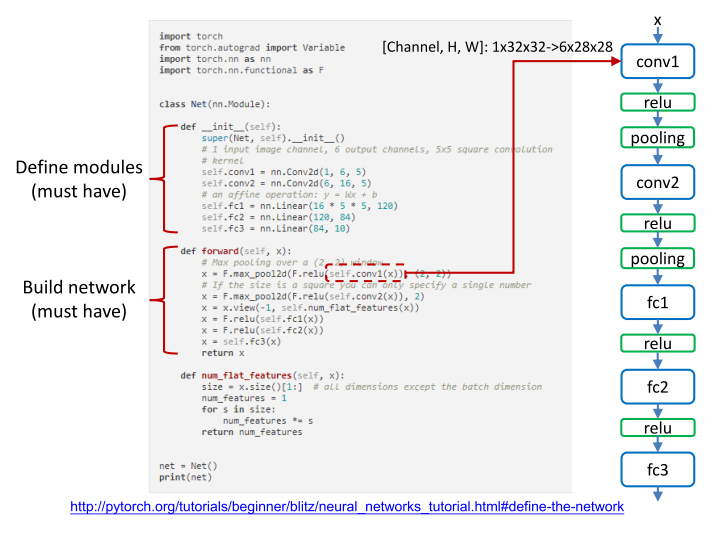
\includegraphics[width=0.8\linewidth,keepaspectratio]{pyt8}
\end{center}

\end{frame}

%%%%%%%%%%%%%%%%%%%%%%%%%%%%%%%%%%%%%%%%%%%%%%%%%%%
\begin{frame}[fragile] \frametitle{How CNN Works}
\begin{center}
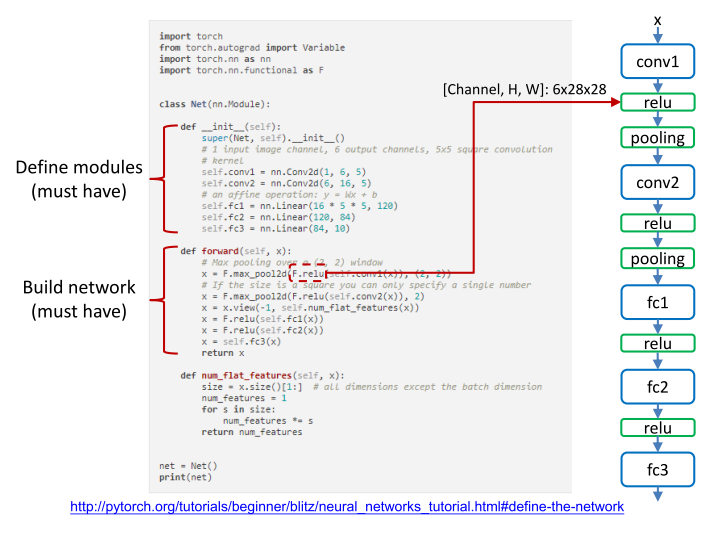
\includegraphics[width=0.8\linewidth,keepaspectratio]{pyt9}
\end{center}

\end{frame}

%%%%%%%%%%%%%%%%%%%%%%%%%%%%%%%%%%%%%%%%%%%%%%%%%%%
\begin{frame}[fragile] \frametitle{How CNN Works}
\begin{center}
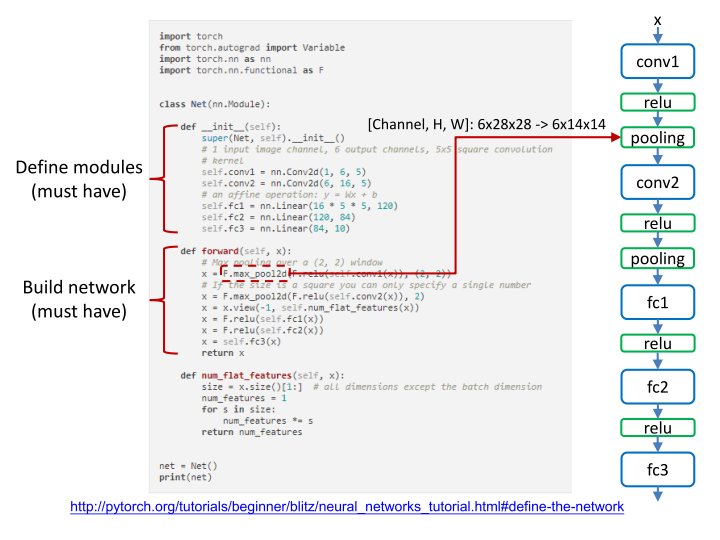
\includegraphics[width=0.8\linewidth,keepaspectratio]{pyt10}
\end{center}

\end{frame}

%%%%%%%%%%%%%%%%%%%%%%%%%%%%%%%%%%%%%%%%%%%%%%%%%%%
\begin{frame}[fragile] \frametitle{How CNN Works}
\begin{center}
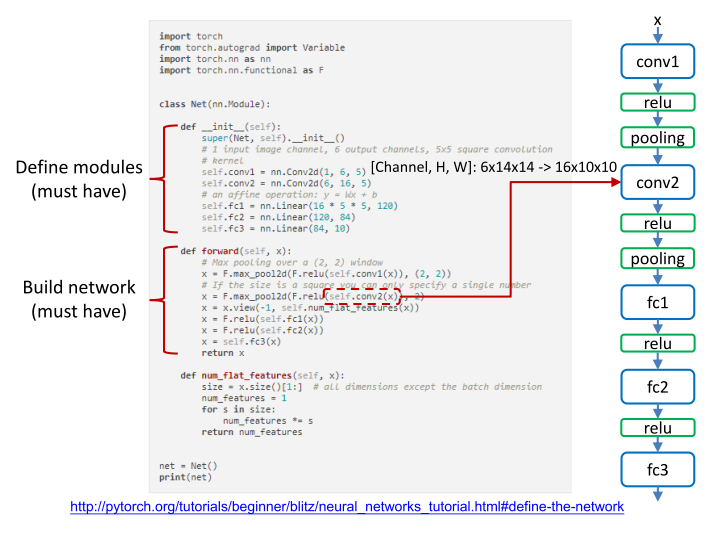
\includegraphics[width=0.8\linewidth,keepaspectratio]{pyt11}
\end{center}

\end{frame}

%%%%%%%%%%%%%%%%%%%%%%%%%%%%%%%%%%%%%%%%%%%%%%%%%%%
\begin{frame}[fragile] \frametitle{How CNN Works}
\begin{center}
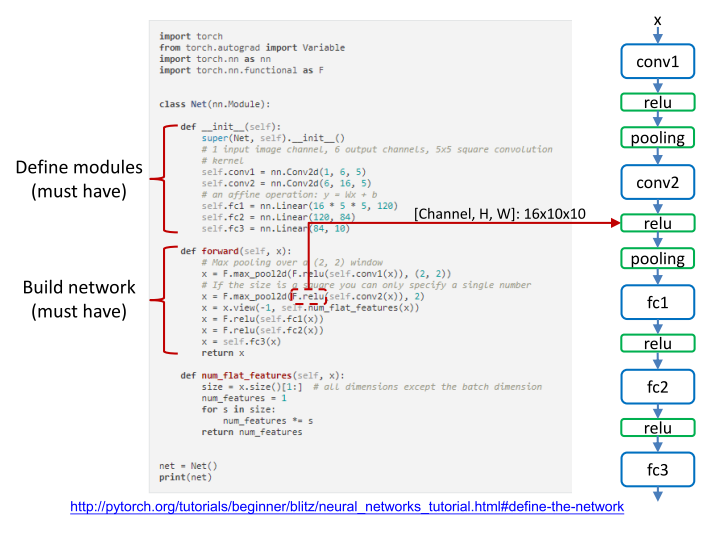
\includegraphics[width=0.8\linewidth,keepaspectratio]{pyt12}
\end{center}

\end{frame}

%%%%%%%%%%%%%%%%%%%%%%%%%%%%%%%%%%%%%%%%%%%%%%%%%%%
\begin{frame}[fragile] \frametitle{How CNN Works}
\begin{center}
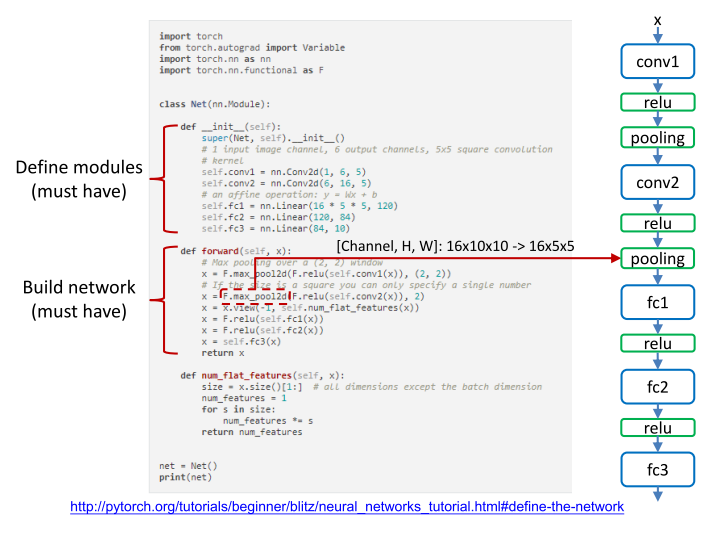
\includegraphics[width=0.8\linewidth,keepaspectratio]{pyt13}
\end{center}

\end{frame}

%%%%%%%%%%%%%%%%%%%%%%%%%%%%%%%%%%%%%%%%%%%%%%%%%%%
\begin{frame}[fragile] \frametitle{How CNN Works}
\begin{center}
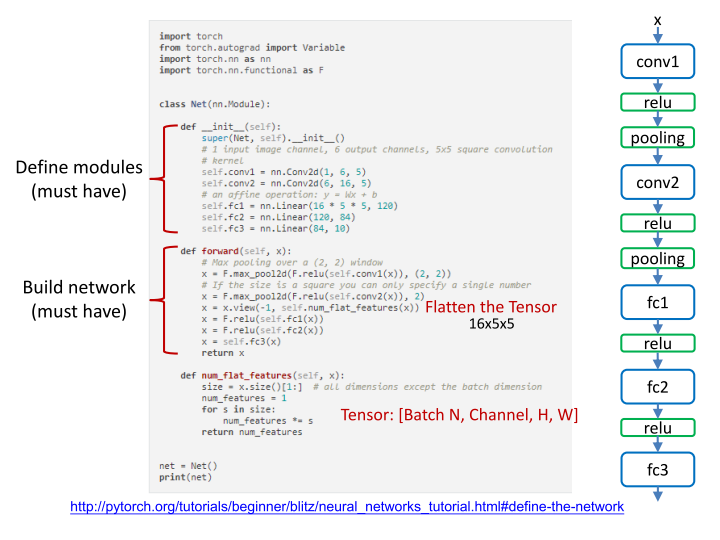
\includegraphics[width=0.8\linewidth,keepaspectratio]{pyt14}
\end{center}

\end{frame}

%%%%%%%%%%%%%%%%%%%%%%%%%%%%%%%%%%%%%%%%%%%%%%%%%%%
\begin{frame}[fragile] \frametitle{How CNN Works}
\begin{center}
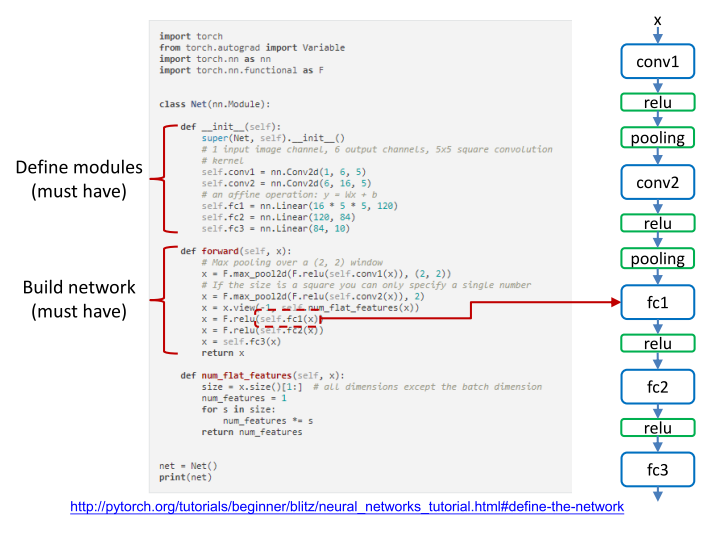
\includegraphics[width=0.8\linewidth,keepaspectratio]{pyt15}
\end{center}

\end{frame}

%%%%%%%%%%%%%%%%%%%%%%%%%%%%%%%%%%%%%%%%%%%%%%%%%%%
\begin{frame}[fragile] \frametitle{How CNN Works}
\begin{center}
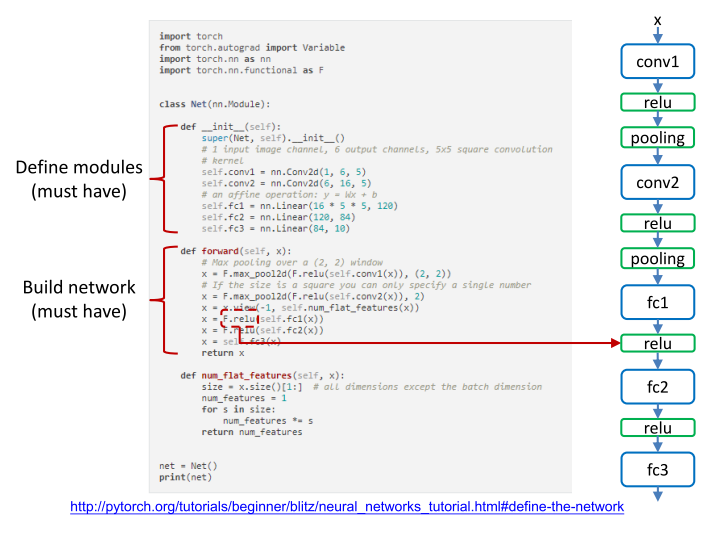
\includegraphics[width=0.8\linewidth,keepaspectratio]{pyt16}
\end{center}

\end{frame}

%%%%%%%%%%%%%%%%%%%%%%%%%%%%%%%%%%%%%%%%%%%%%%%%%%%
\begin{frame}[fragile] \frametitle{How CNN Works}
\begin{center}
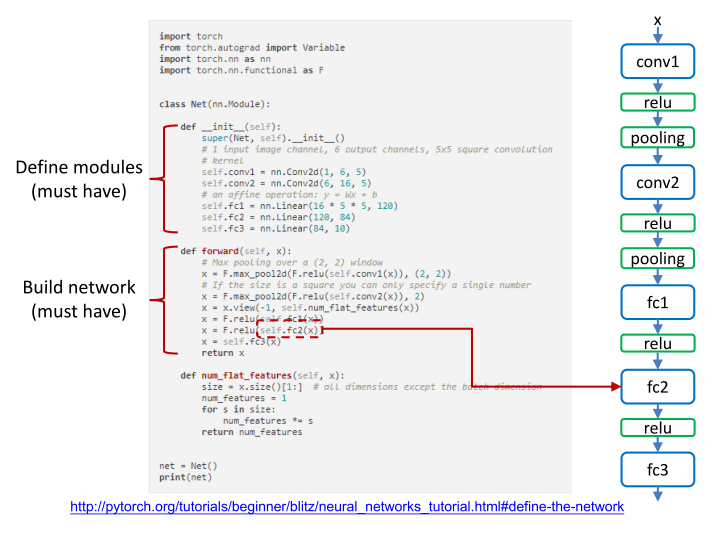
\includegraphics[width=0.8\linewidth,keepaspectratio]{pyt17}
\end{center}

\end{frame}

%%%%%%%%%%%%%%%%%%%%%%%%%%%%%%%%%%%%%%%%%%%%%%%%%%%
\begin{frame}[fragile] \frametitle{How CNN Works}
\begin{center}
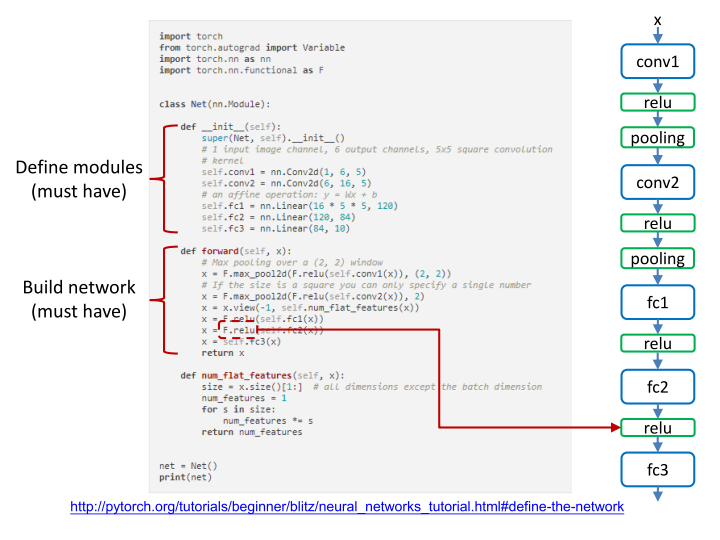
\includegraphics[width=0.8\linewidth,keepaspectratio]{pyt18}
\end{center}

\end{frame}

%%%%%%%%%%%%%%%%%%%%%%%%%%%%%%%%%%%%%%%%%%%%%%%%%%%
\begin{frame}[fragile] \frametitle{How CNN Works}
\begin{center}
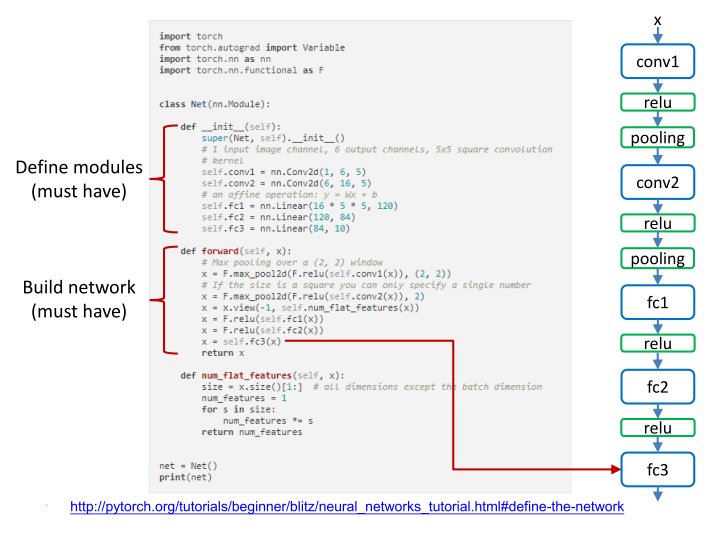
\includegraphics[width=0.8\linewidth,keepaspectratio]{pyt19}
\end{center}
\tiny{(Reference:PyTorch Tutorial-NTU Machine Learning Course-Lyman Lin )}
\end{frame}
